\documentclass[english]{beamer}
%\usepackage{beamerarticle}
\usepackage{graphicx}
\usepackage{babel}
\usepackage{tikz}
\usetikzlibrary{arrows,shapes}
\usepackage[all]{xy}
\usepackage[invisible]{arxiv-beamer-theme}

\usepackage[utf8]{inputenc}
%%%
%%% Natbib must be here!! (after Beamer stuff)
\usepackage[authoryear,square]{natbib}
\usepackage{amsmath}
\usepackage{amsthm}
\usepackage{amsfonts}
\usepackage{amssymb}
% \usepackage{bbm}  % Para el \bb{1}
\usepackage{multidef}
\usepackage{verbatim}
% \usepackage{stmaryrd} %% para \llbracket
%%
%% \usepackage[bottom=2cm, top=2cm, left=2cm, right=2cm]{geometry}
%% \usepackage{titling}
%% \setlength{\droptitle}{-10ex} 
%%
\renewcommand{\o}{\vee}
\renewcommand{\O}{\bigvee}
\newcommand{\y}{\wedge}
\newcommand{\Y}{\bigwedge}
\newcommand{\limp}{\longrightarrow}
\newcommand{\lsii}{\longleftrightarrow}
%%

\DeclareMathOperator{\cf}{cf}
\DeclareMathOperator{\dom}{domain}
\DeclareMathOperator{\im}{img}
\DeclareMathOperator{\Fn}{Fn}
\DeclareMathOperator{\rk}{rk}
\DeclareMathOperator{\mos}{mos}
\DeclareMathOperator{\trcl}{trcl}
\DeclareMathOperator{\Con}{Con}
\DeclareMathOperator{\Club}{Club}


\newcommand{\modelo}[1]{\mathbf{#1}}
\newcommand{\axiomas}[1]{\mathit{#1}}
\newcommand{\clase}[1]{\mathsf{#1}}
\newcommand{\poset}[1]{\mathbb{#1}}
\newcommand{\operador}[1]{\mathbf{#1}}

%% \newcommand{\Lim}{\clase{Lim}}
%% \newcommand{\Reg}{\clase{Reg}}
%% \newcommand{\Card}{\clase{Card}}
%% \newcommand{\On}{\clase{On}}
%% \newcommand{\WF}{\clase{WF}}
%% \newcommand{\HF}{\clase{HF}}
%% \newcommand{\HC}{\clase{HC}}
%%
%% El siguiente comando reemplaza todos los anteriores:
%%
\multidef{\clase{#1}}{Card,HC,HF,Lim,On->Ord,Reg,WF,Ord}
\newcommand{\ON}{\On}

%% En lugar de usar todo el paquete bbm:
\DeclareMathAlphabet{\mathbbm}{U}{bbm}{m}{n} 
\renewcommand{\1}{\mathbbm{1}}
\newcommand{\PP}{\mathbbm{P}}

%%
%% \newcommand{\calD}{\mathcal{D}}
%% \newcommand{\calS}{\mathcal{S}}
%% \newcommand{\calU}{\mathcal{U}}
%% \newcommand{\calB}{\mathcal{B}}
%% \newcommand{\calL}{\mathcal{L}}
%% \newcommand{\calF}{\mathcal{F}}
%% \newcommand{\calT}{\mathcal{T}}
%% \newcommand{\calW}{\mathcal{W}}
%% \newcommand{\calA}{\mathcal{A}}
%%
%% El siguiente comando reemplaza todos los anteriores:
%%
\multidef[prefix=cal]{\mathcal{#1}}{A-Z}
%%
%% \newcommand{\A}{\modelo{A}}
%% \newcommand{\BB}{\modelo{B}}
%% \newcommand{\ZZ}{\modelo{Z}}
%% \newcommand{\PP}{\modelo{P}}
%% \newcommand{\QQ}{\modelo{Q}}
%% \newcommand{\RR}{\modelo{R}}
%%
%% El siguiente comando reemplaza todos los anteriores:
%%
\multidef{\modelo{#1}}{A,BB->B,CC->C,NN->N,QQ->Q,RR->R,ZZ->Z}

\multidef[prefix=p]{\mathbb{#1}}{A-Z}
%% \newcommand{\B}{\modelo{B}}
%% \newcommand{\C}{\modelo{C}}
%% \newcommand{\F}{\modelo{F}}
%% \newcommand{\D}{\modelo{D}}

\newcommand{\Th}{\mb{Th}}
\newcommand{\Mod}{\mb{Mod}}

\newcommand{\Se}{\operador{S^\prec}}
\newcommand{\Pu}{\operador{P_u}}
\renewcommand{\Pr}{\operador{P_R}}
\renewcommand{\H}{\operador{H}}
\renewcommand{\S}{\operador{S}}
\newcommand{\I}{\operador{I}}
\newcommand{\E}{\operador{E}}

\newcommand{\se}{\preccurlyeq}
\newcommand{\ee}{\succ}
\newcommand{\id}{\approx}
\newcommand{\subm}{\subseteq}
\newcommand{\ext}{\supseteq}
\newcommand{\iso}{\cong}
%%
\renewcommand{\emptyset}{\varnothing}
\newcommand{\rel}{\mathcal{R}}
\newcommand{\Pow}{\mathop{\mathcal{P}}}
\renewcommand{\P}{\Pow}
\newcommand{\BP}{\mathrm{BP}}
\newcommand{\func}{\rightarrow}
\newcommand{\ord}{\mathrm{Ord}}
\newcommand{\R}{\mathbb{R}}
\newcommand{\N}{\mathbb{N}}
\newcommand{\Z}{\mathbb{Z}}
\renewcommand{\I}{\mathbb{I}}
\newcommand{\Q}{\mathbb{Q}}
\newcommand{\B}{\mathbf{B}}
\newcommand{\lb}{\langle}
\newcommand{\rb}{\rangle}
\newcommand{\impl}{\rightarrow}
\newcommand{\ent}{\Rightarrow}
\newcommand{\tne}{\Leftarrow}
\newcommand{\sii}{\Leftrightarrow}
\renewcommand{\phi}{\varphi}
\newcommand{\phis}{{\varphi^*}}
\renewcommand{\th}{\theta}
\newcommand{\Lda}{\Lambda}
\newcommand{\La}{\Lambda}
\newcommand{\lda}{\lambda}
\newcommand{\ka}{\kappa}
\newcommand{\del}{\delta}
\newcommand{\de}{\delta}
\newcommand{\ze}{\zeta}
%\newcommand{\ }{\ }
\newcommand{\la}{\lambda}
\newcommand{\al}{\alpha}
\newcommand{\be}{\beta}
\newcommand{\ga}{\gamma}
\newcommand{\Ga}{\Gamma}
\newcommand{\ep}{\varepsilon}
\newcommand{\De}{\Delta}
\newcommand{\defi}{\mathrel{\mathop:}=}
\newcommand{\forces}{\Vdash}
%\newcommand{\ap}{\mathbin{\wideparen{\ }}}
\newcommand{\Tree}{{\mathrm{Tr}_\N}}
\newcommand{\PTree}{{\mathrm{PTr}_\N}}
\newcommand{\NWO}{\mathit{NWO}}
\newcommand{\Suc}{{\N^{<\N}}}%
\newcommand{\init}{\mathsf{i}}
\newcommand{\ap}{\mathord{^\smallfrown}}
\newcommand{\Cantor}{\mathcal{C}}
%\newcommand{\C}{\Cantor}
\newcommand{\Baire}{\mathcal{N}}
\newcommand{\sig}{\ensuremath{\sigma}}
\newcommand{\fsig}{\ensuremath{F_\sigma}}
\newcommand{\gdel}{\ensuremath{G_\delta}}
\newcommand{\Sig}{\ensuremath{\boldsymbol{\Sigma}}}
\newcommand{\bPi}{\ensuremath{\boldsymbol{\Pi}}}
\newcommand{\Del}{\ensuremath{\boldsymbol\Delta}}
%\renewcommand{\F}{\operador{F}}
\newcommand{\ths}{{\theta^*}}
\newcommand{\om}{\ensuremath{\omega}}
%\renewcommand{\c}{\complement}
\newcommand{\comp}{\mathsf{c}}
\newcommand{\co}[1]{\left(#1\right)^\comp}
\newcommand{\len}[1]{\left|#1\right|}
\DeclareMathOperator{\tlim}{\overline{\mathrm{TLim}}}
\newcommand{\card}[1]{{\left|#1\right|}}
\newcommand{\bigcard}[1]{{\bigl|#1\bigr|}}
%
% Cardinality
%
\newcommand{\lec}{\leqslant_c}
\newcommand{\gec}{\geqslant_c}
\newcommand{\lc}{<_c}
\newcommand{\gc}{>_c}
\newcommand{\eqc}{=_c}
\newcommand{\biy}{\approx}
\newcommand*{\ale}[1]{\aleph_{#1}}
%
\newcommand{\Zerm}{\axiomas{Z}}
\newcommand{\ZC}{\axiomas{ZC}}
\newcommand{\AC}{\axiomas{AC}}
\newcommand{\DC}{\axiomas{DC}}
\newcommand{\MA}{\axiomas{MA}}
\newcommand{\CH}{\axiomas{CH}}
\newcommand{\ZFC}{\axiomas{ZFC}}
\newcommand{\ZF}{\axiomas{ZF}}
\newcommand{\Inf}{\axiomas{Inf}}
%
% Cardinal characteristics
%
\newcommand{\cont}{\mathfrak{c}}
\newcommand{\spl}{\mathfrak{s}}
\newcommand{\bound}{\mathfrak{b}}
\newcommand{\mad}{\mathfrak{a}}
\newcommand{\tower}{\mathfrak{t}}
%
\renewcommand{\hom}[2]{{}^{#1}\hskip-0.116ex{#2}}
\newcommand{\pred}[1][{}]{\mathop{\mathrm{pred}_{#1}}}
%% Postfix operator with supressable space:
%% \newcommand*{\iseg}{\relax\ifnum\lastnodetype>0 \mskip\medmuskip\fi{\downarrow}} %
\newcommand*{\iseg}{{\downarrow}}
\newcommand{\rr}{\mathrel{R}}
\newcommand{\restr}{\upharpoonright}
%\newcommand{\type}{\mathtt{}}
\newcommand{\app}{\mathop{\mathrm{Aprox}}}
\newcommand{\hess}{\triangleleft}
\newcommand{\bx}{\bar{x}}
\newcommand{\by}{\bar{y}}
\newcommand{\bz}{\bar{z}}
\newcommand{\union}{\mathop{\textstyle\bigcup}}
\newcommand{\sm}{\setminus}
\newcommand{\sbq}{\subseteq}
\newcommand{\nsbq}{\subseteq}
\newcommand{\mty}{\emptyset}
\newcommand{\dimg}{\text{\textup{``}}} % direct image
\newcommand{\quine}[1]{\ulcorner{\!#1\!}\urcorner}
%\newcommand{\ntrm}[1]{\textsl{\textbf{#1}}}
\newcommand{\Null}{\calN\!\mathit{ull}}
\DeclareMathOperator{\club}{Club}
\DeclareMathOperator{\otp}{otp}
\DeclareMathOperator{\val}{\mathit{val}}
\DeclareMathOperator{\chk}{\mathit{check}}
\DeclareMathOperator{\edrel}{\mathit{edrel}}
\DeclareMathOperator{\eclose}{\mathit{eclose}}
\DeclareMathOperator{\Memrel}{\mathit{Memrel}}
\renewcommand{\PP}{\mathbb{P}}
\renewcommand{\app}{\mathrm{App}}
\newcommand{\formula}{\isatt{formula}}
\newcommand{\tyi}{\isatt{i}}
\newcommand{\tyo}{\isatt{o}}
\newcommand{\forceisa}{\mathop{\mathtt{forces}}}
\newcommand{\equ}{\mathbf{e}}
\newcommand{\bel}{\mathbf{b}}
\newcommand{\atr}{\mathit{atr}}
\newcommand{\concat}{\mathbin{@}}
\newcommand{\dB}[1]{\mathbf{#1}}
\newcommand{\ed}{\mathrel{\isatt{ed}}}
\newcommand{\frecR}{\mathrel{\isatt{frecR}}}
\newcommand{\forceseq}{\mathop{\isatt{forces{\isacharunderscore}eq}}}
\newcommand{\forcesmem}{\mathop{\isatt{forces{\isacharunderscore}mem}}}
\newcommand{\forcesat}{\mathop{\isatt{forces{\isacharunderscore}at}}}
\newcommand{\pleq}{\preceq}


%%%%%%%%%%%%%%%%%%%%%%%%%
% Variant aleph, beth, etc
% From http://tex.stackexchange.com/q/170476/69595
\makeatletter
\@ifpackageloaded{txfonts}\@tempswafalse\@tempswatrue
\if@tempswa
  \DeclareFontFamily{U}{txsymbols}{}
  \DeclareFontFamily{U}{txAMSb}{}
  \DeclareSymbolFont{txsymbols}{OMS}{txsy}{m}{n}
  \SetSymbolFont{txsymbols}{bold}{OMS}{txsy}{bx}{n}
  \DeclareFontSubstitution{OMS}{txsy}{m}{n}
  \DeclareSymbolFont{txAMSb}{U}{txsyb}{m}{n}
  \SetSymbolFont{txAMSb}{bold}{U}{txsyb}{bx}{n}
  \DeclareFontSubstitution{U}{txsyb}{m}{n}
  \DeclareMathSymbol{\aleph}{\mathord}{txsymbols}{64}
  \DeclareMathSymbol{\beth}{\mathord}{txAMSb}{105}
  \DeclareMathSymbol{\gimel}{\mathord}{txAMSb}{106}
  \DeclareMathSymbol{\daleth}{\mathord}{txAMSb}{107}
\fi
\makeatother

%%%%%%%%%%%%%%%%%%%%%%%%%%%%%%%%%%%%%%%%%%%%%%%%%%%%%%%%%%%%
%%
%% Theorem Environments
%%
% \newtheorem{theorem}{Theorem}
% \newtheorem{lemma}[theorem]{Lemma}
% \newtheorem{prop}[theorem]{Proposition}
% \newtheorem{corollary}[theorem]{Corollary}
% \newtheorem{claim}{Claim}
% \newtheorem*{claim*}{Claim}
% \theoremstyle{definition}
% \newtheorem{definition}[theorem]{Definition}
% \newtheorem{remark}[theorem]{Remark}
% \newtheorem{example}[theorem]{Example}
% \theoremstyle{remark}
% \newtheorem*{remark*}{Remark}

%%%%%%%%%%%%%%%%%%%%%%%%%%%%%%%%%%%%%%%%%%%%%%%%%%%%%%%%%%%%%%%%%%%%%%

%% \newenvironment{inducc}{\begin{list}{}{\itemindent=2.5em \labelwidth=4em}}{\end{list}}
%% \newcommand{\caso}[1]{\item[\fbox{#1}]}
\newenvironment{proofofclaim}{\begin{proof}[Proof of Claim]}{\end{proof}}

\newcommand{\quantRel}[3]{#1 #2\kern -1pt[#3]}
\newcommand{\forallRel}[2]{\quantRel{\forall}{#1}{#2}}
\newcommand{\existsRel}[2]{\quantRel{\exists}{#1}{#2}}


%%% Local Variables: 
%%% mode: latex
%%% TeX-master: "forcing_IJCAR2020_slides"
%%% End: 

\usepackage{isabelle,isabellesym}
\newcommand{\uscore}{\isacharunderscore}

\CompileMatrices

\title[Forcing in Isabelle/ZF]{Formalization of Forcing in Isabelle/ZF}

\author[E.~Gunther, M.~Pagano, PST]{E.~Gunther \qquad M.~Pagano \qquad P.~Sánchez Terraf\thanks{Supported by
    CONICET and SeCyT-UNC} 
}
\institute[UNC]{CIEM-FaMAF --- Universidad Nacional de Córdoba}

\date[IJCAR 2020]{International Joint Conference on Automated
  Reasoning\\ Paris (Virtual),\ \  2020 / 07 / 02}

\subject{Logic in Computer Science}

\pgfdeclareimage[height=3ex]{UNC-logo}{unc_400_Blanco_Negro}
\logo{\pgfuseimage{UNC-logo}}

%% Para usar overlays con tikz
\tikzset{onslide/.code args={<#1>#2}{%
    \only<#1>{\pgfkeysalso{#2}} % \pgfkeysalso doesn't change the path
}}

\begin{document}

\begin{frame}[plain]
  \titlepage
  \begin{center}
    \insertlogo
  \end{center}
\end{frame}
%
\begin{frame}
  \frametitle{Summary}
  \tableofcontents
  \transwipe
\end{frame}
%
%%%%%%%%%%%%%%%%%%%%%%%%%%%%%%%%%%%%%%%%%%%%%%%%%%%
\section{Introduction}

%-%-%-%-%-%-%-%-%-%-%-%-%-%-%-%-%-%-%-%-%-%-%-%-%-%
\subsection{Why Isabelle/ZF?}

\begin{frame}
  \frametitle{Why Isabelle/ZF?}
  \begin{block}{Pros}
    \begin{itemize}
    \item Most advanced set theory formalized (around 2017).
    \item Structured proof language Isar
      \citep{DBLP:conf/tphol/Wenzel99}.
    \item Comparatively low in consistency strength.
    \end{itemize}
  \end{block}
  %
  \pause
  %
  \begin{block}{Cons}
    \begin{itemize}
    \item A fraction of automation of Isabelle (\texttt{sledgehammer},
      etc).
    \item ``Untyped'', and too weak a metatheory.
    \end{itemize}
  \end{block}
\end{frame}

\begin{frame}
  \frametitle{Isabelle/ZF \citep{DBLP:journals/jar/PaulsonG96}}
  \begin{itemize}
  \item<.-> An object logic of Isabelle axiomatized over the
    intuitionistic fragment  \emph{Pure} of higher order logic.
  \item<+-> It postulates two types: \isatt{i}
    (sets) and \isatt{o} (booleans). \visible<3->{\alert{Not
      inductively defined!}}
  \item<+-> The Replacement and Separation axiom schemes feature free
    high order variables.
  \item<+-> Induction/recursion is \emph{internal} to the theory (it works as a
    layer on top of set-theoretical proofs of well-foundedness (of
    $\N$, of $\Ord$, etc).
  \end{itemize}
\end{frame}

%-%-%-%-%-%-%-%-%-%-%-%-%-%-%-%-%-%-%-%-%-%-%-%-%-%
\subsection{The ctm approach to forcing}

\begin{frame}
  \frametitle{The ctm approach to forcing, 1/4}
  \begin{block}{Countable transitive model (ctm) of $\ZF$}
    $\lb M, E\rb \models \ZF$ where
    \begin{itemize}
    \item \alert<3>{$M$ is \emph{standard}:\quad $E \defi {\in}\restriction M$.}
    \item $M$ is countable, and \emph{transitive}:\quad $x\in y \in M \implies x\in M$.
    \end{itemize}
  \end{block}
  %
  \pause%
  %
  \textbf{Note}. If $\lb N, R\rb \models \ZF$ with $R$ well-founded, then there
  exists a ctm $M$ of $\ZF$.
  \pause

  It makes sense to compare, for $x,y\in M$:
  \[
  x \sbq y
  \begin{overlayarea}{4.5em}{2ex}
    \ \ \ \only<3-4>{\ \  and}\only<5>{\alert{$\iff$}}
  \end{overlayarea}
  M \models x\sbq y
  \]
  \pause
  The rhs can be written as a term of type \isatt{o}:

  {} \hfill   $\forall z.\ z\in M \longrightarrow (z\in x \longrightarrow z\in
  y)$,
  \hfill the \textbf{relativization} $\sbq^M$ of $\sbq$ to $M$. 
  \pause

  In this case, we know that  $\sbq$  is \textbf{absolute for
    transitive models}.
\end{frame}

\begin{frame}
  \frametitle{The ctm approach to forcing, 2/4}
  Let $\lb \PP, {\preceq} ,\1\rb \in M$ be a \emph{forcing notion} (a preorder with top). Given 
  an \emph{$M$-generic} filter $G\sbq \PP$, 
  we can adjoin it to $M$ to form the
  \textbf{generic extension} $M[G]$.
  \pause

  Every $a\in M[G]$ is coded by
  some $\punto{a}\in M$ through the function $\val$:
  \[
  M[G]\defi \{ \val(G,\punto{a}) : \punto{a}\in M\}
  \]
  Fundamentally, \textbf{truth} in $M[G]$ is coded in $M$ by the
  function $\forceisa$.
  \pause
  \begin{theorem}[\citep{Cohen-CH-PNAS}]
    \begin{enumerate}
    \item $\forceisa$ is definable over $M$.
      %
    \item For every $\phi$, $M$-generic $G$, and $\punto{a}\in M$,
      \[
      M[G], [\val(G,\punto{a})] \models \phi
      \quad      \iff  \quad 
      \exists p\in G.\ \; M, [p,\preceq,\PP, \punto{a}]  \models
      \forceisa(\phi).
      \]
      \pause
      \rule{21em}{0pt}
      \raisebox{1.6ex}[0ex]{$\overset{\searrow}{}$ \ \ 
        $p \alert{\forces^M_{\PP,\preceq}} \phi(\punto{a})$
        \  \ $\overset{\swarrow}{}$}
    \end{enumerate}
  \end{theorem} 
\end{frame}

\begin{frame}
  \frametitle{The ctm approach to forcing, 3/4}
  \begin{block}{Benefits of using ctms}
    \begin{enumerate}
    \item<+-> Countability ensures that generics exist (by
      Rasiowa-Sikorski Lemma).
      %  
    \item<+-> Absoluteness provides seamless
      treatment of many concepts.
      \begin{center}
        $\alpha$ is an ordinal \ $\iff$ \  $M\models \alpha$ is
        an ordinal \  $\iff$ \  $M[G]\models \alpha$ is an ordinal
      \end{center}
      %
    \item<+-> Both $M$ and $M[G]$ are standard (two-valued) models.
      %
    \item<+-> Ctms are
      used in an important (perhaps the greatest) fraction of the literature.
    \end{enumerate}
  \end{block}
\end{frame}

\begin{frame}
  \frametitle{The ctm approach to forcing, 4/4}
  By choosing  $\lb \PP, {\preceq} ,\1\rb$
  appropriately one can tune the first order properties of  $M[G]$ (for
  any generic $G$).
  \pause
  %
  \begin{theorem}[\citep{Cohen-CH-PNAS}]
    If $\PP$ is the set of finite partial binary functions with domain
    included in $\aleph_2^M$, $M[G]$ satisfies the negation of the
    \textbf{Continuum Hypothesis} ($\CH$):
    \[
    M[G] \models 2^{\aleph_0} >\aleph_1.
    \]
  \end{theorem}
  \pause
  
  Formalizing the independence of $\CH$ from the axioms of $\ZFC$
  using ctms is one of the main goals of our project.
\end{frame}

%-%-%-%-%-%-%-%-%-%-%-%-%-%-%-%-%-%-%-%-%-%-%-%-%-%
\subsection{Other approaches}
\begin{frame}
  \frametitle{Other approaches to set theory and forcing}
  \begin{itemize}
  \item<+-> \alert{Lean}: Full formalization of the Boolean-valued approach to
    forcing and the independence of $\CH$ \citep{DBLP:conf/cpp/HanD20}.
  \item<+-> Set theory over Isabelle/HOL:
    \begin{itemize}
    \item \isatt{HOLZF} \citep{DBLP:conf/ictac/Obua06}
    \item \isatt{ZFC{\uscore}in{\uscore}HOL}
      \citep{ZFC_in_HOL-AFP}
    \end{itemize}
  \end{itemize}
  %
  \begin{block}{A word on consistency strength}<+->
    \begin{description}
      \setlength{\labelwidth}{12em}
      \setlength{\labelsep}{2em}
      \setlength{\itemindent}{6em}
    \item[Isabelle/ZF + ctm]  (far) less than $\ZF$ +  one
      inaccessible.
    \item[\isatt{HOLZF},
      \isatt{ZFC{\uscore}in{\uscore}HOL}]
      approximately $\ZF$ +  one   inaccessible. 
    \item[Lean (CiC)] $\ZF$ + $\omega$ inaccessibles \citep{carneiro-ms-thesis}. 
    \end{description}
  \end{block}
\end{frame}

%%%%%%%%%%%%%%%%%%%%%%%%%%%%%%%%%%%%%%%%%%%%%%%%%%%
\section{The development}

%-%-%-%-%-%-%-%-%-%-%-%-%-%-%-%-%-%-%-%-%-%-%-%-%-%
\subsection{What did we accomplish?}

\begin{frame}
  \frametitle{What did we accomplish?}
  %
  \begin{shadowblock}{}
    \begin{enumerate}
    \item<1-> We adapted the \texttt{ZF-Constructible} library
      \citep{paulson_2003} to obtain
      absoluteness results for nonempty transitive classes ($\to$
      \alert{Isabelle2020}).
    \item<2-> We formalized the formula transformer $\forceisa$ and
      hence the forcing relation $\forces$, and proved the Fundamental
      Theorems.
    \item<3-> We showed that generic extensions of ctms of $\ZF$ are also
      ctms of $\ZF$ (respectively, adding $\AC$).
    \item<4-> We provided the forcing notion that adds a Cohen real,
      therefore proving the existence of a nontrivial extension.
    \end{enumerate}
  \end{shadowblock}
\end{frame}

\begin{frame}
  \frametitle{Some details}
  \begin{alertblock}{}
    \begin{enumerate}%\setcounter{enumi}{1}
    \item We adapted \texttt{ZF-Constructible} to obtain
      sharper absoluteness results.
    \end{enumerate}
  \end{alertblock}

  This library originally contains a major development of relativization and
  absoluteness for \emph{classes} $C :: {}$ \isatt{i} $\Rightarrow$
  \isatt{o}, including the definition of the set \isatt{formula} ::
  \isatt{i} of internal formulas and model theoretic satisfaction. 
  \pause
  \begin{block}{Relativization and synthesis discipline}
    \begin{enumerate}[I]
    \item<+-> $p=\{x,y\} :: {}$\isatt{i}
      \hfill
      (original term).
    \item<+-> \isatt{upair}$(C,x,y,p) :: {}$\isatt{o}
      \hfill
      (relativization, fully
      relational). 
    \item<+-> \isatt{upair{\uscore}fm}$(0,1,2) :: {}$\isatt{i} 
      \hfill
      (synthesized member of \isatt{formula}).
    \end{enumerate}
  \end{block}
  \begin{alertblock}{}<+->
    Around 40 absoluteness/closure lemmas now hold using weaker
    hypotheses on the class $C$ (most of them, just that $C$ is
    transitive and nonempty).
  \end{alertblock}
\end{frame}

\begin{frame}{Some details}
  \begin{alertblock}{}
    \begin{enumerate}\setcounter{enumi}{1}
    \item We formalized the formula transformer $\forceisa$ and
      hence the forcing relation $\forces$, and proved the Fundamental
      Theorems.
    \end{enumerate}
  \end{alertblock}
  %
  \pause
  %
  \begin{block}{$\;\forceisa$ is defined by recursion on  formulas}
    This is the main reason we work with the set of internalized
    formulas, and that we require legit first-order expressions for
    the axiom schemes (Separation and Replacement).

    The base cases  $\forceisa(x\in y)$ and  $\forceisa(x =
    y)$ are  defined by \alert{internal} well-founded
    recursion.
  \end{block}
  %
  \pause
  \begin{alertblock}{}
    We enhanced the recursion results of Isabelle/ZF as well as
    the relevant preservation results in ZF-Constructible, thus
    showing that forcing is absolute for atomic formulas.
  \end{alertblock}
\end{frame}

\begin{frame}{Some details}
  \begin{alertblock}{}
    \begin{enumerate}\setcounter{enumi}{2}
    \item For any ctm $M$ of $\ZF$ and $M$-generic $G$, $M[G] \models
      \ZF$ (respectively, adding $\AC$).
    \end{enumerate}
  \end{alertblock}
  \pause
  Actually, the modularity of the theory of forcing allowed us to do
  this \alert{before} we write down the definition of $\forceisa$.
  \pause
  
  We may compare some of the code with the actual
  math \citep{kunen2011set}.
\end{frame}

%-%-%-%-%-%-%-%-%-%-%-%-%-%-%-%-%-%-%-%-%-%-%-%-%-%
\subsection{Math vs Code}

\begin{frame}<1-12>[label=code-review]
  \begin{center}\setlength{\fboxsep}{0pt}
    \only<01>{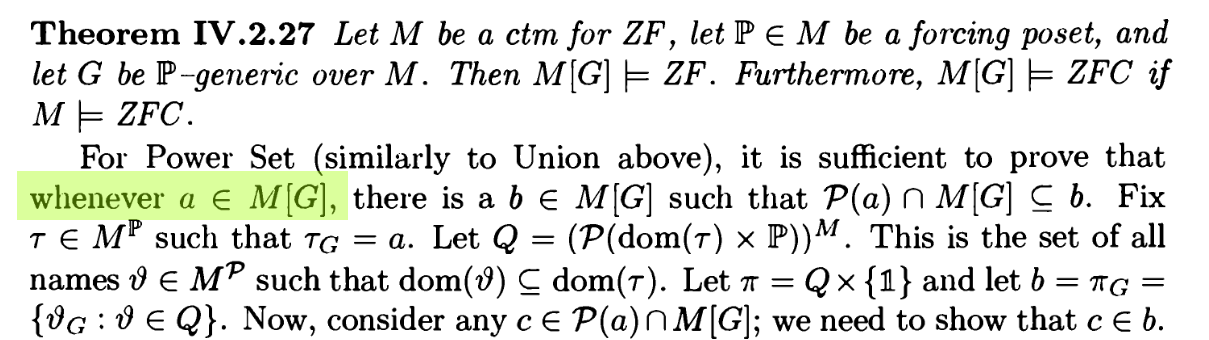
\includegraphics[scale=0.23]{kunen_powerset_01.png} \\ \fbox{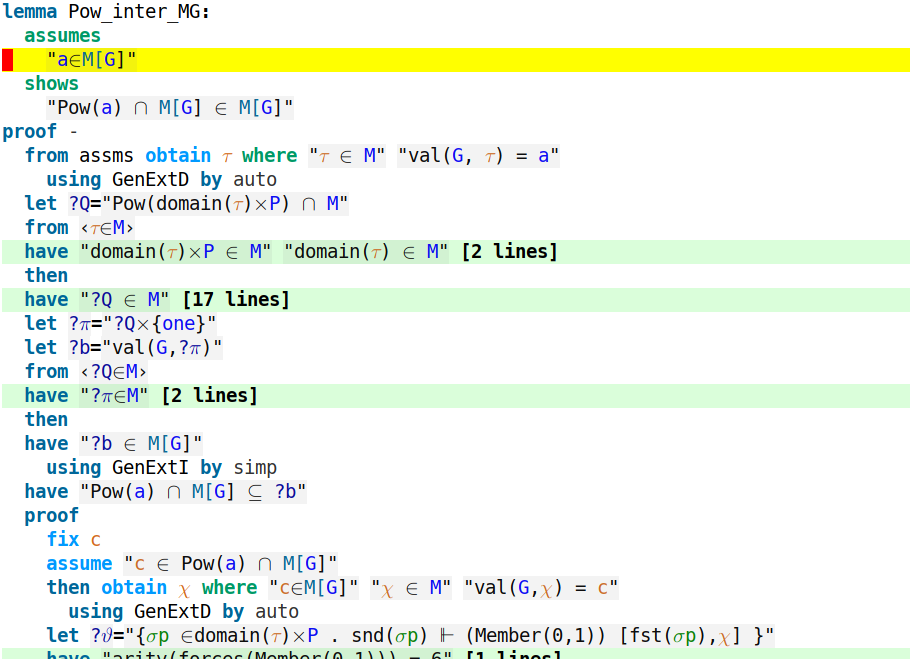
\includegraphics[scale=0.26]{isa_converted_01.png}}}%
    \only<02>{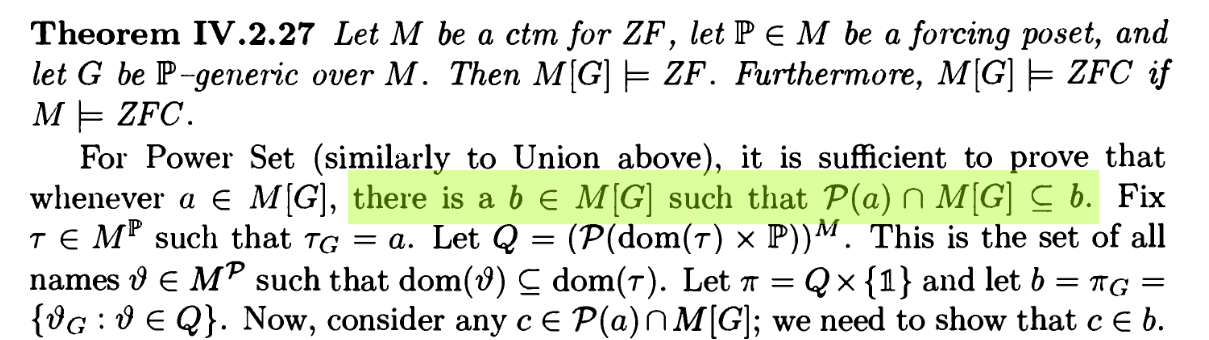
\includegraphics[scale=0.23]{kunen_powerset_02.png} \\ \fbox{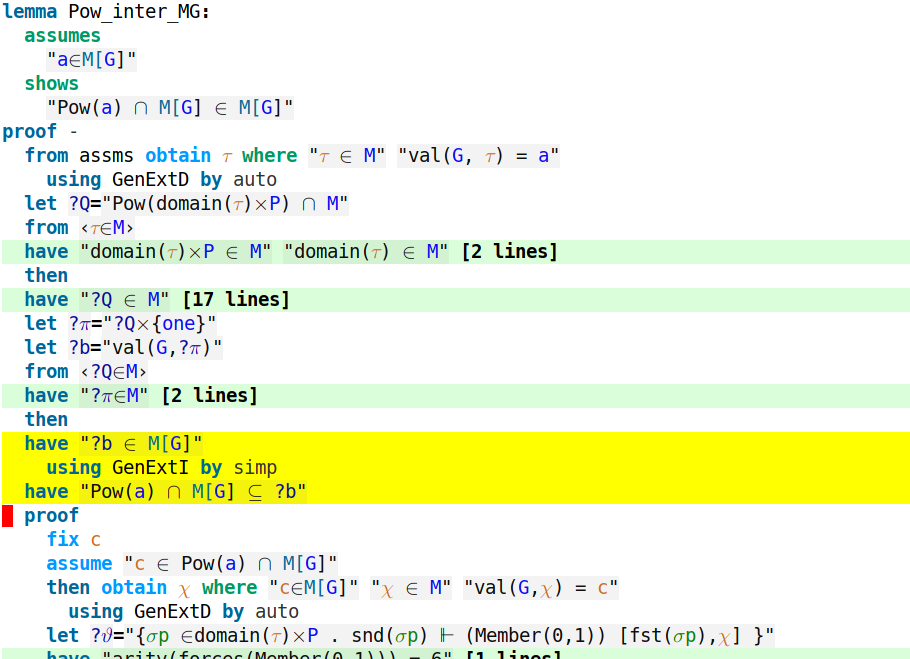
\includegraphics[scale=0.26]{isa_converted_02.png}}}%
    \only<03>{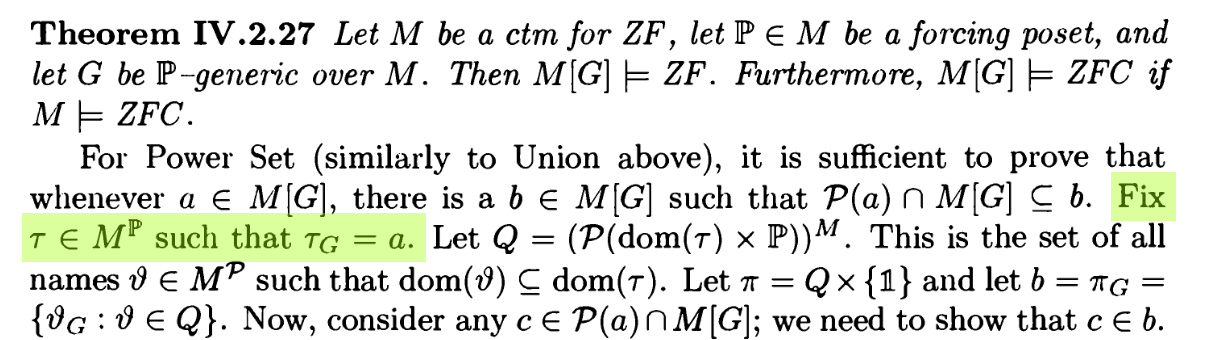
\includegraphics[scale=0.23]{kunen_powerset_03.png} \\ \fbox{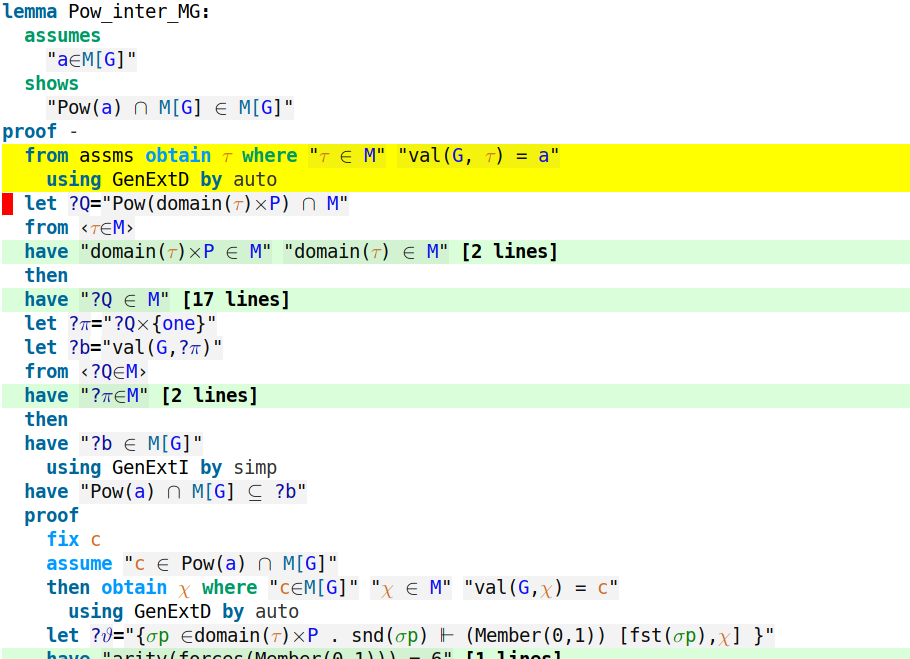
\includegraphics[scale=0.26]{isa_converted_03.png}}}%
    \only<04>{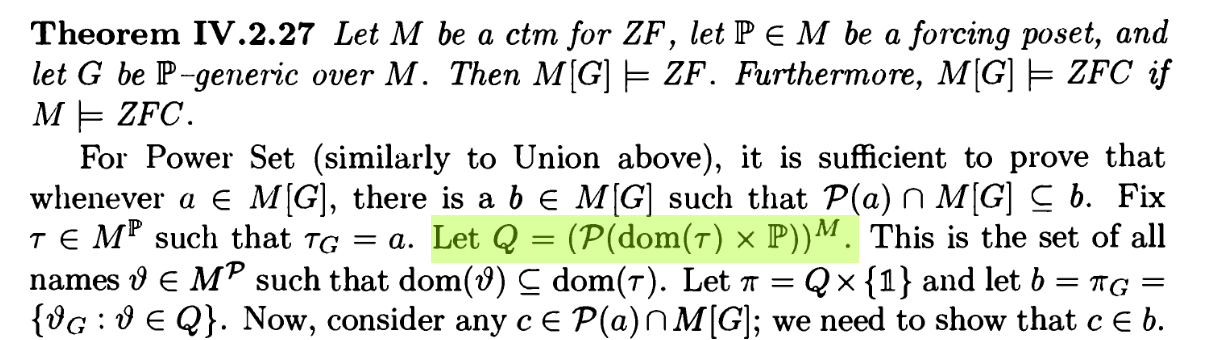
\includegraphics[scale=0.23]{kunen_powerset_04.png} \\ \fbox{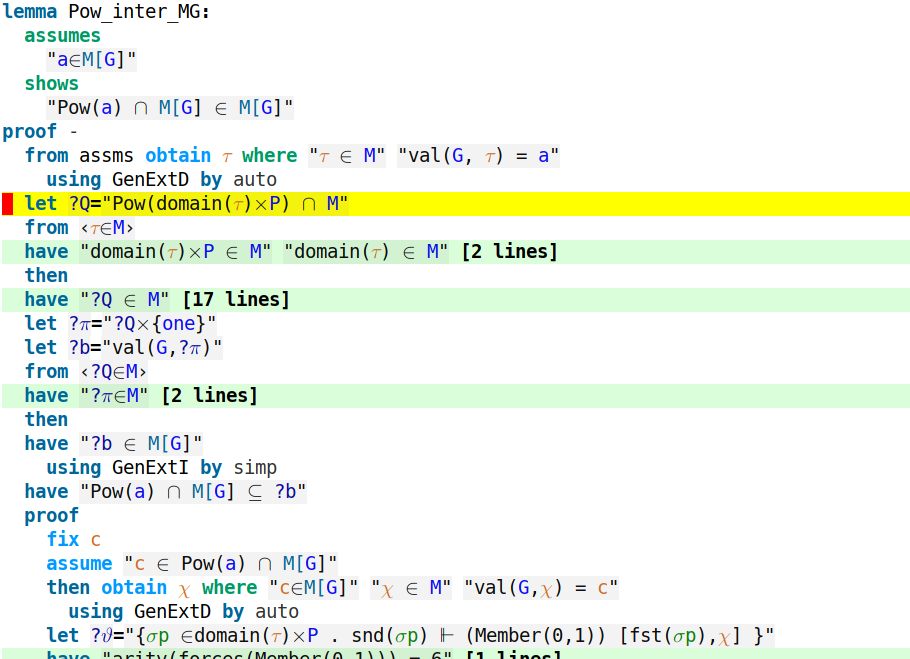
\includegraphics[scale=0.26]{isa_converted_04.png}}}%
    \only<05>{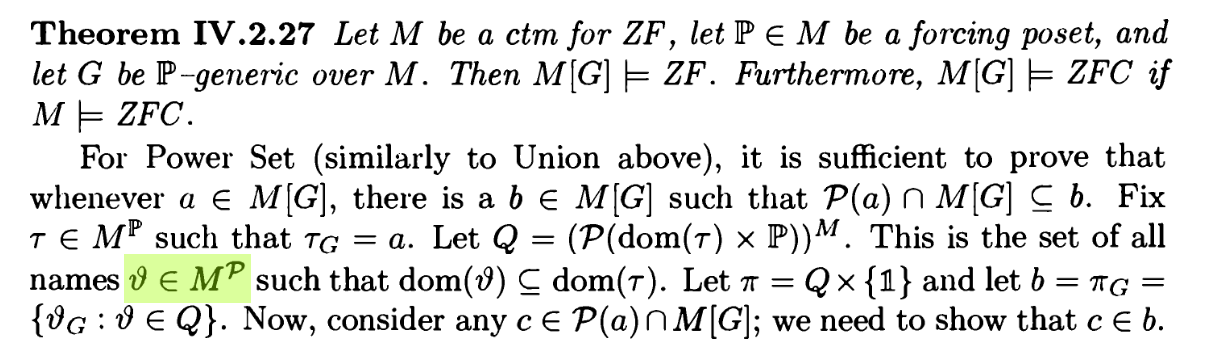
\includegraphics[scale=0.23]{kunen_powerset_05.png} \\ \fbox{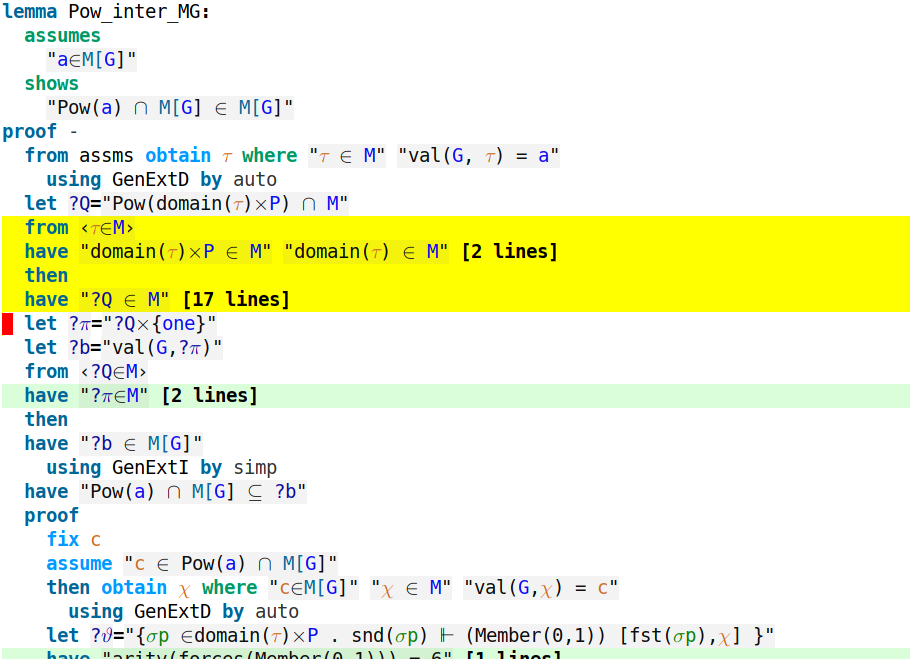
\includegraphics[scale=0.26]{isa_converted_05.png}}}%
    \only<06>{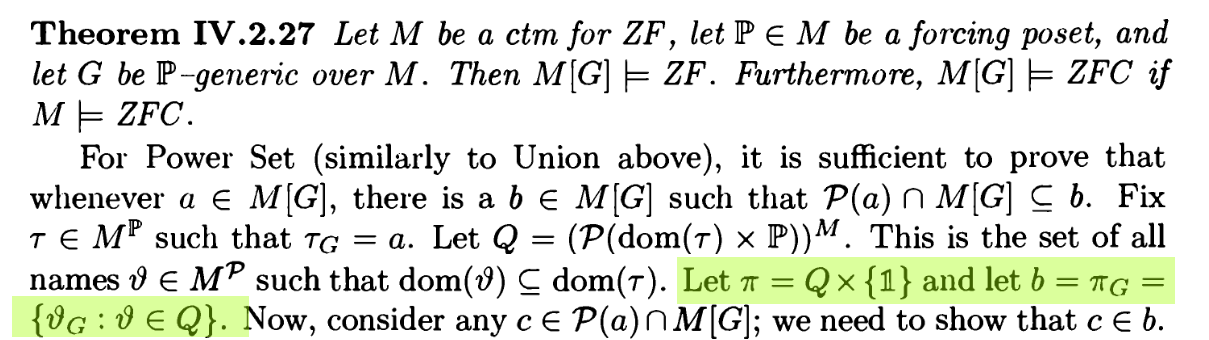
\includegraphics[scale=0.23]{kunen_powerset_06.png} \\ \fbox{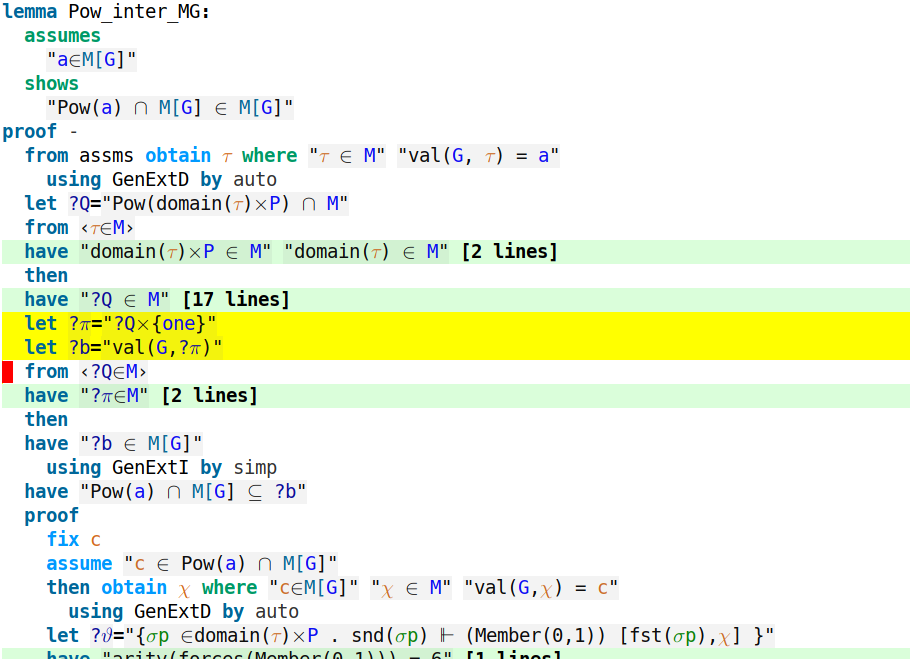
\includegraphics[scale=0.26]{isa_converted_06.png}}}%
    \only<07>{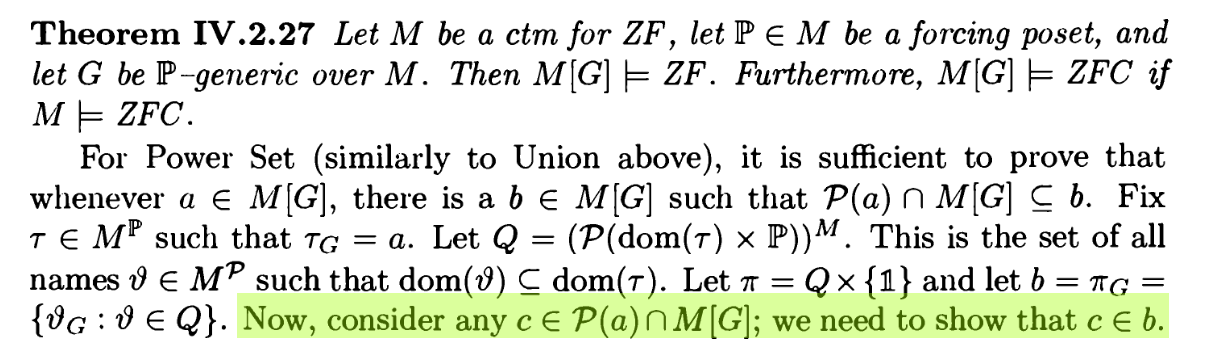
\includegraphics[scale=0.23]{kunen_powerset_07.png} \\ \fbox{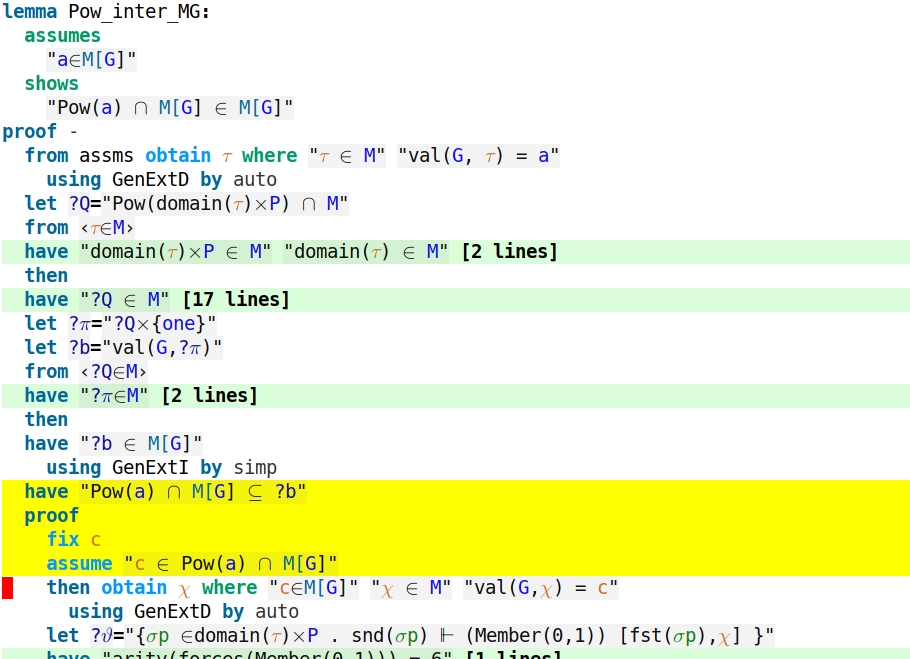
\includegraphics[scale=0.26]{isa_converted_07.png}}}%
    \vspace{3.00115pt}\only<08>{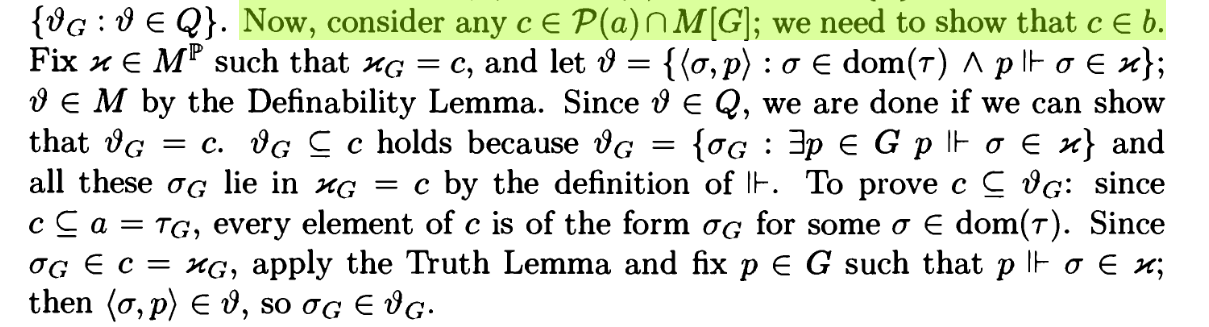
\includegraphics[scale=0.23]{kunen_powerset_08.png} \\ \fbox{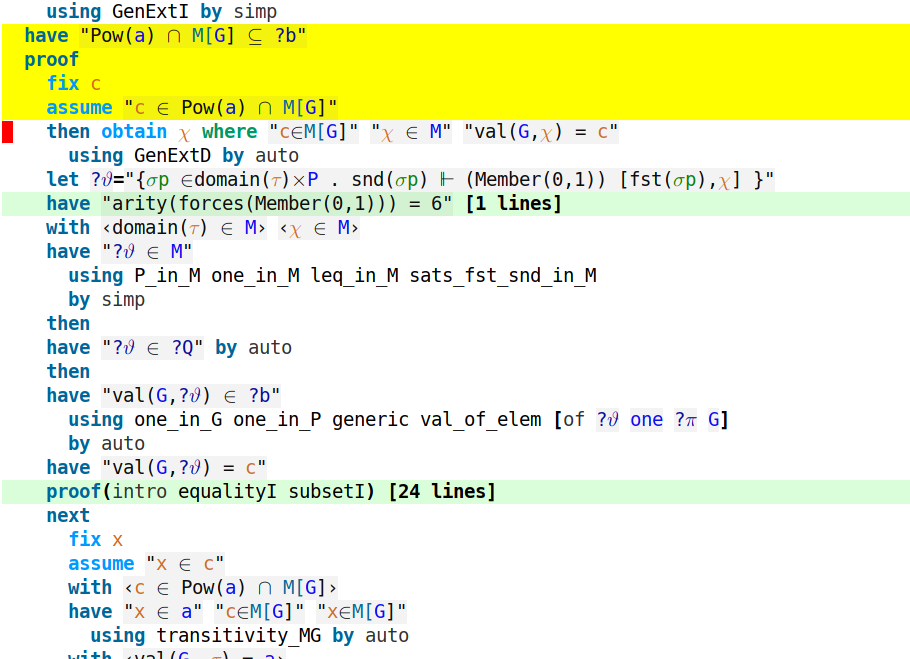
\includegraphics[scale=0.26]{isa_converted_08.png}}}%
    \only<09>{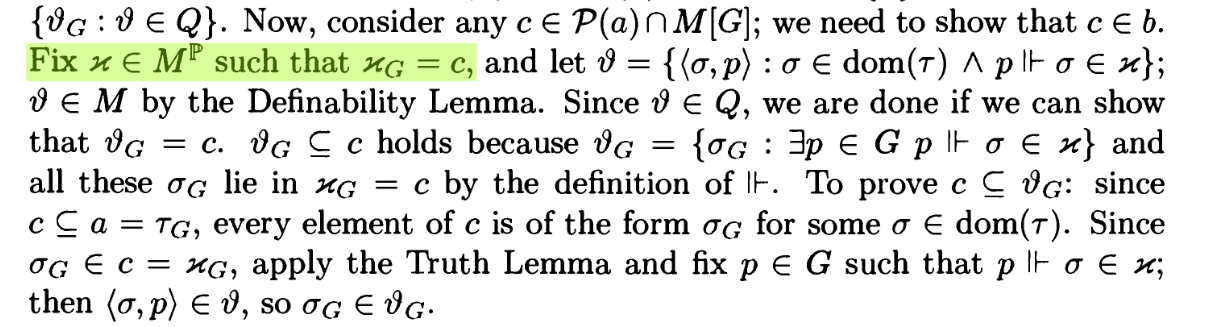
\includegraphics[scale=0.23]{kunen_powerset_09.png} \\ \fbox{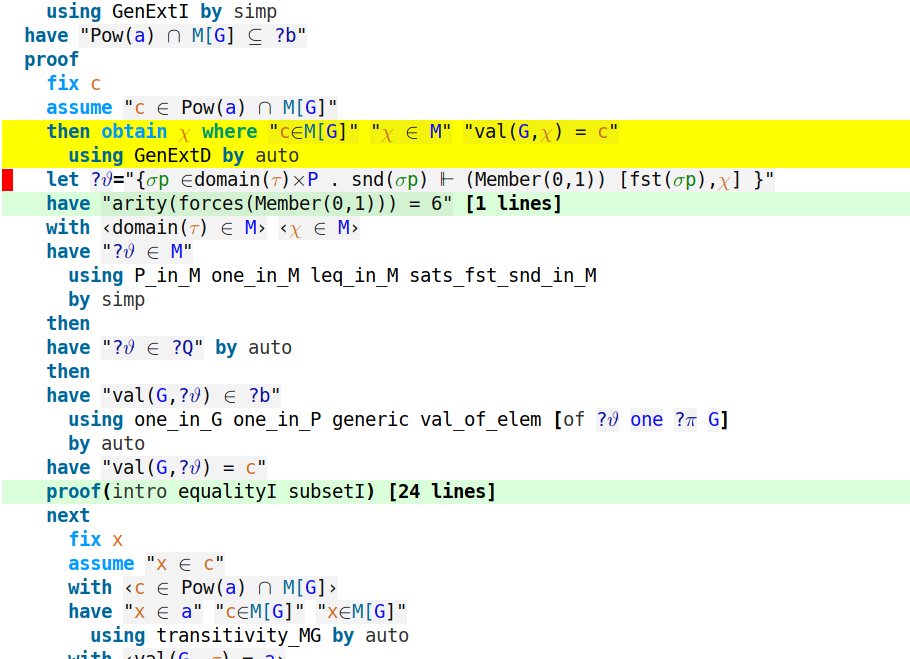
\includegraphics[scale=0.26]{isa_converted_09.png}}}%
    \only<10>{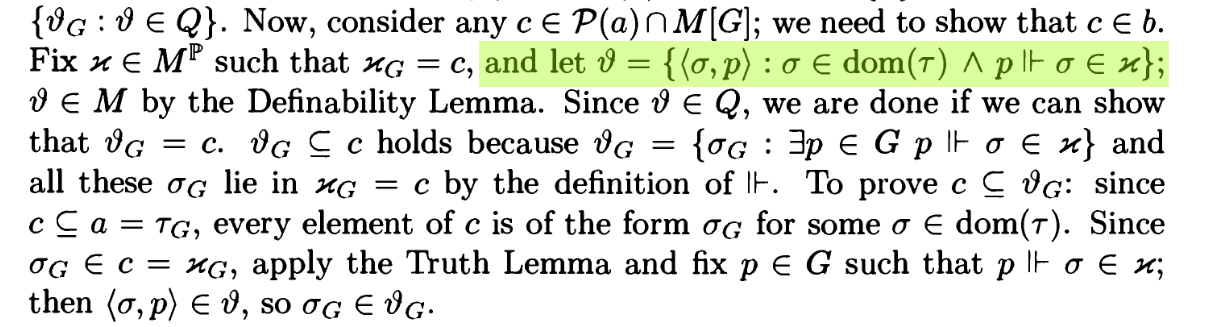
\includegraphics[scale=0.23]{kunen_powerset_10.png} \\ \fbox{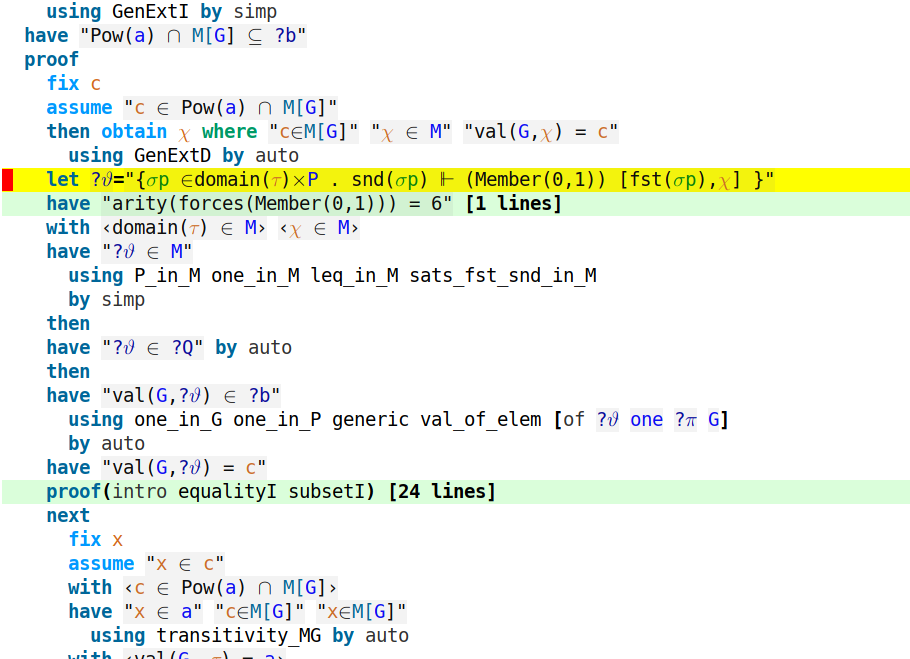
\includegraphics[scale=0.26]{isa_converted_10.png}}}%
    \only<11>{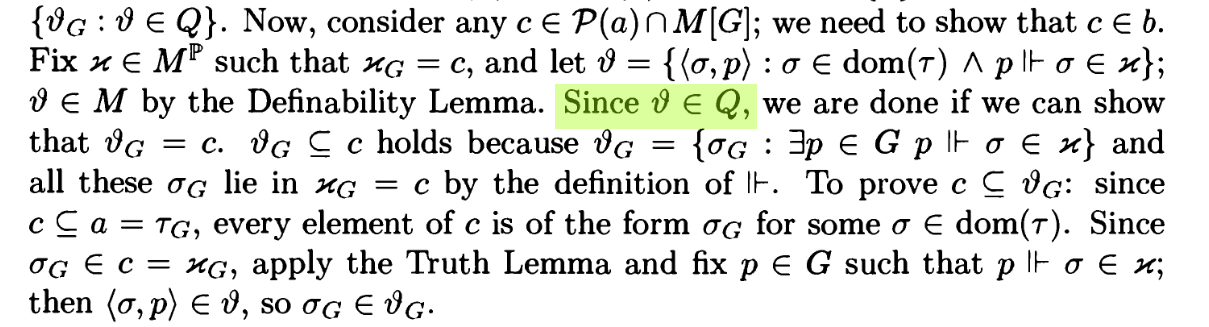
\includegraphics[scale=0.23]{kunen_powerset_11.png} \\ \fbox{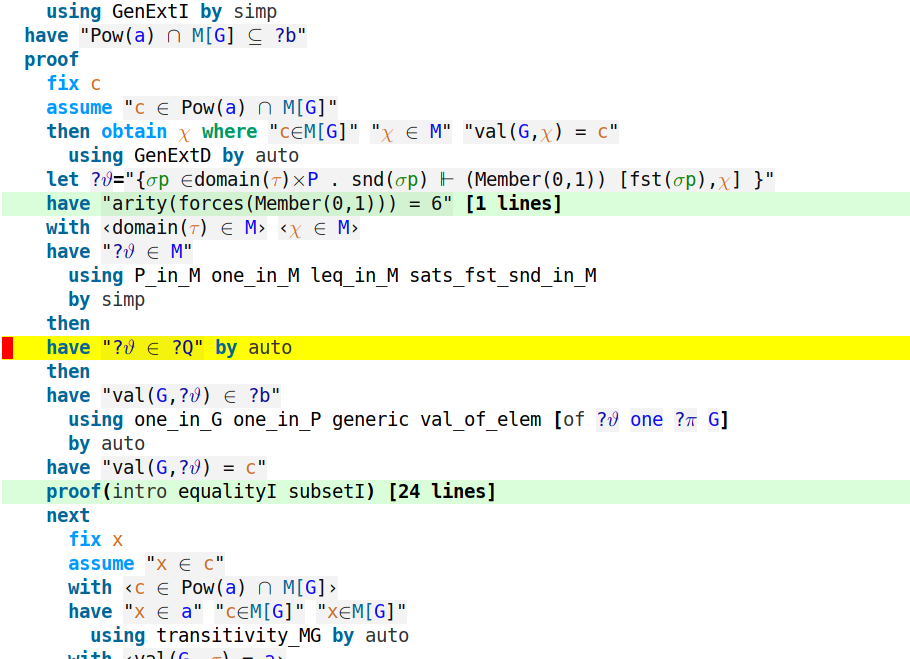
\includegraphics[scale=0.26]{isa_converted_11.png}}}%
    \only<12>{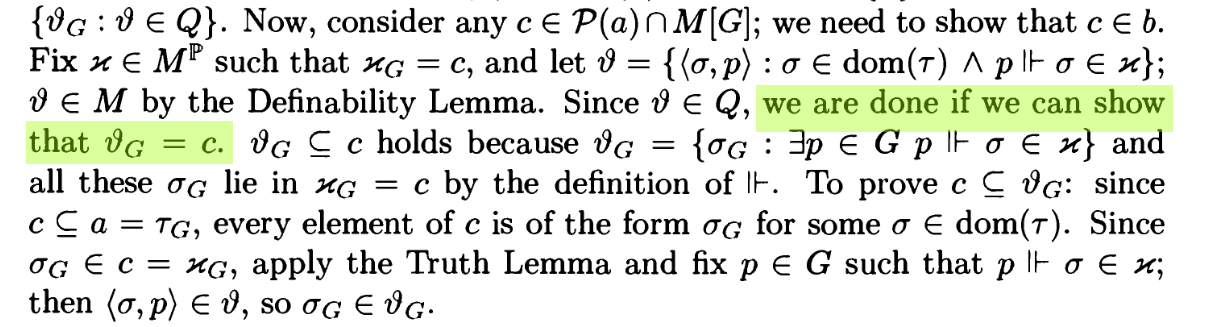
\includegraphics[scale=0.23]{kunen_powerset_12.png} \\ \fbox{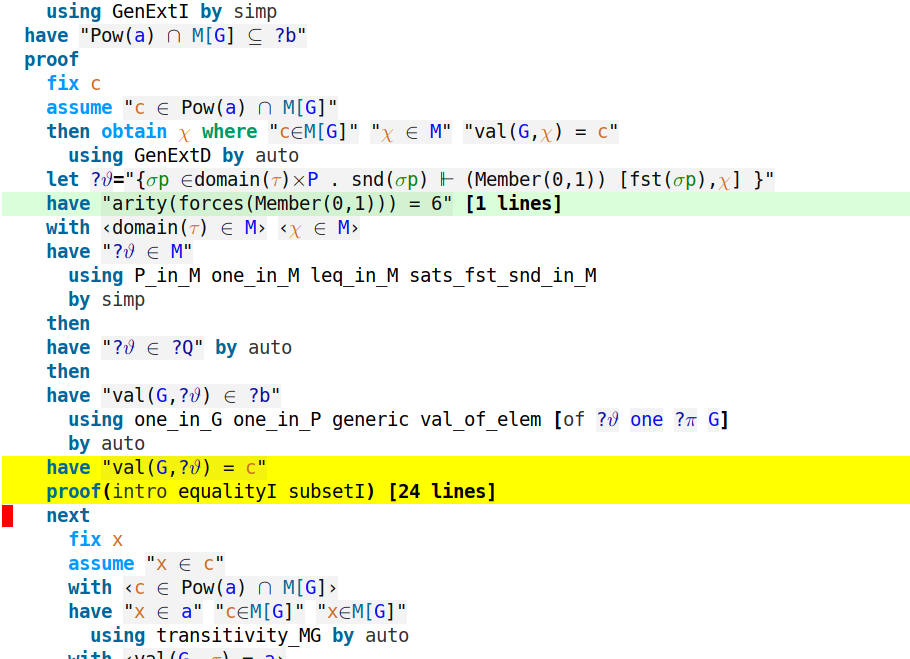
\includegraphics[scale=0.26]{isa_converted_12.png}}}%
    \only<13>{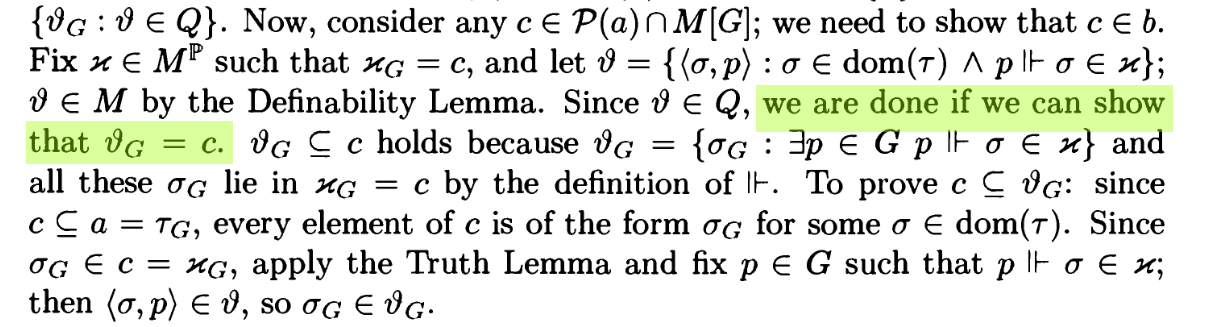
\includegraphics[scale=0.23]{kunen_powerset_13.png} \\ \fbox{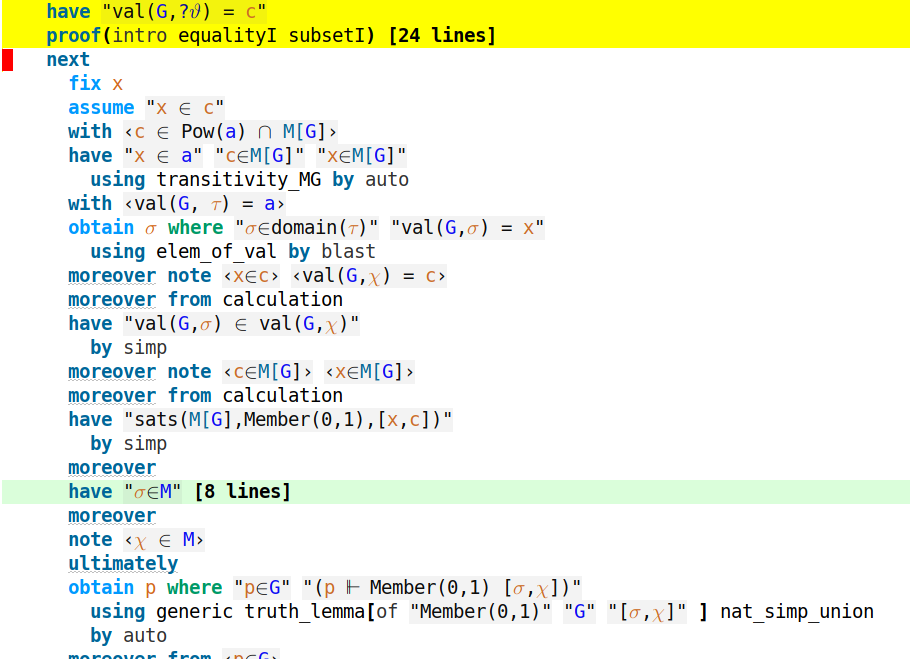
\includegraphics[scale=0.26]{isa_converted_13.png}}}%
    \only<14>{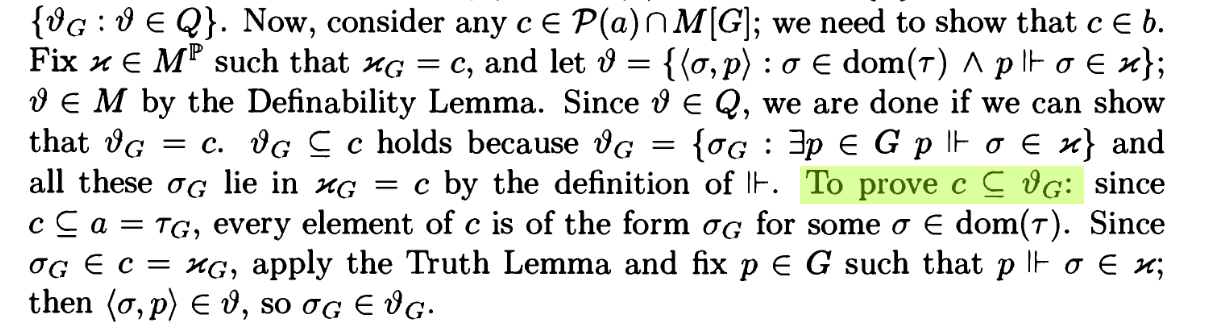
\includegraphics[scale=0.23]{kunen_powerset_14.png} \\ \fbox{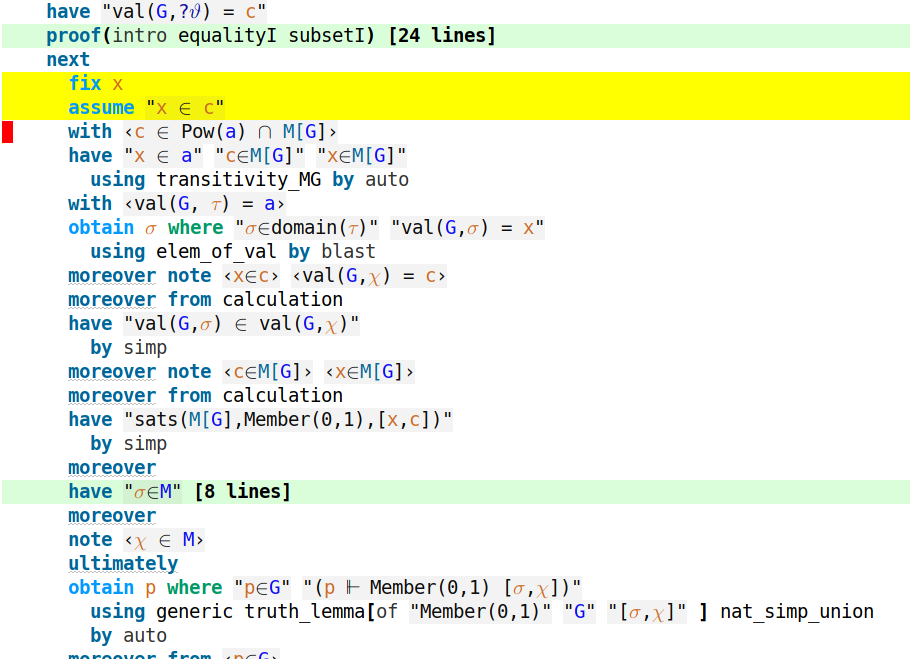
\includegraphics[scale=0.26]{isa_converted_14.png}}}%
    \only<15>{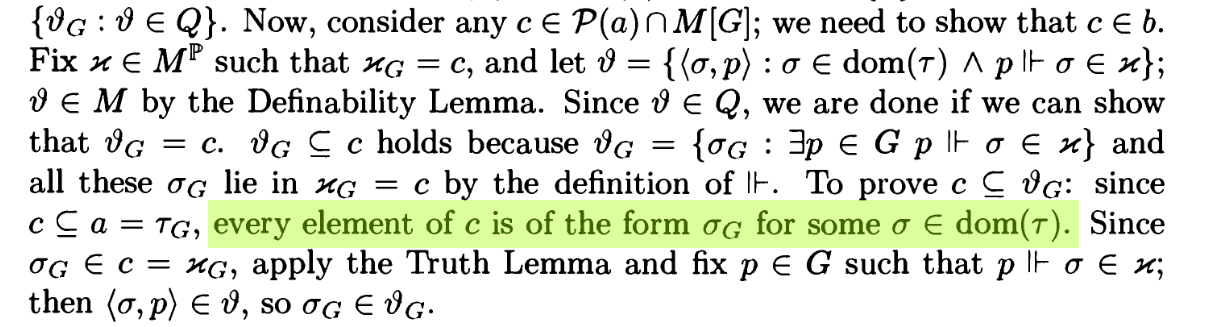
\includegraphics[scale=0.23]{kunen_powerset_15.png} \\ \fbox{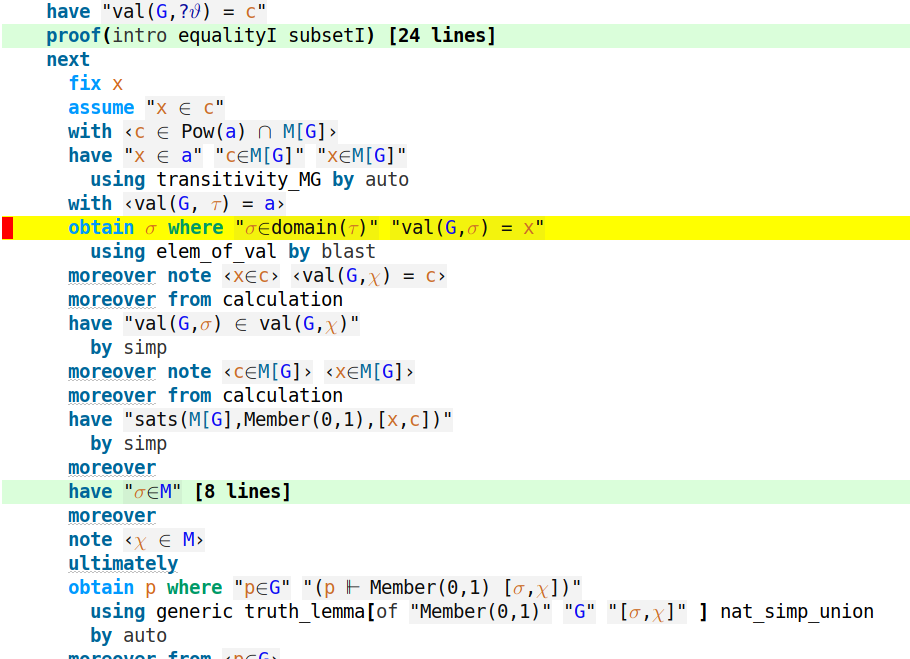
\includegraphics[scale=0.26]{isa_converted_15.png}}}%
    \only<16>{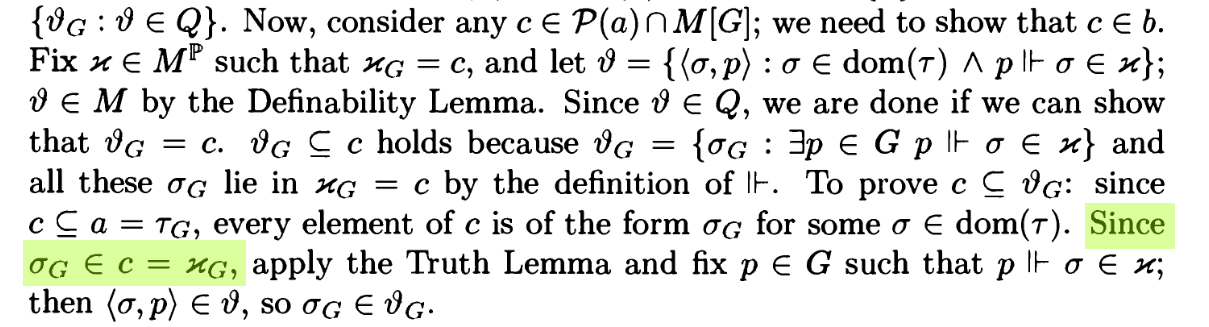
\includegraphics[scale=0.23]{kunen_powerset_16.png} \\ \fbox{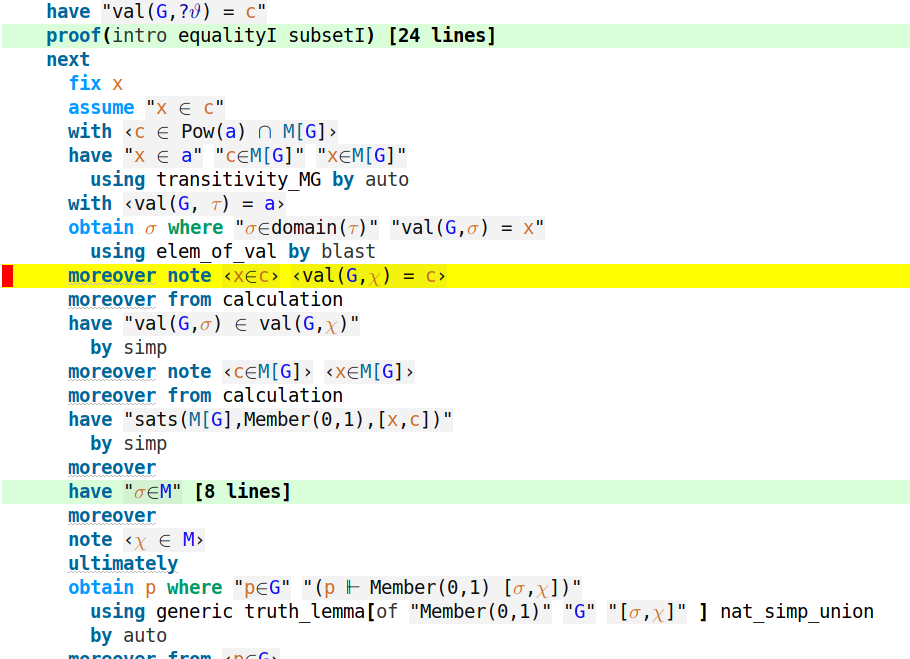
\includegraphics[scale=0.26]{isa_converted_16.png}}}%
    \only<17>{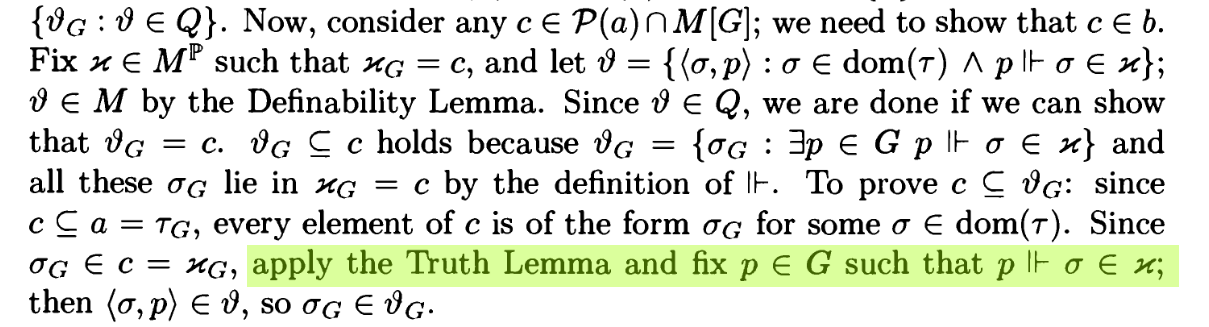
\includegraphics[scale=0.23]{kunen_powerset_17.png} \\ \fbox{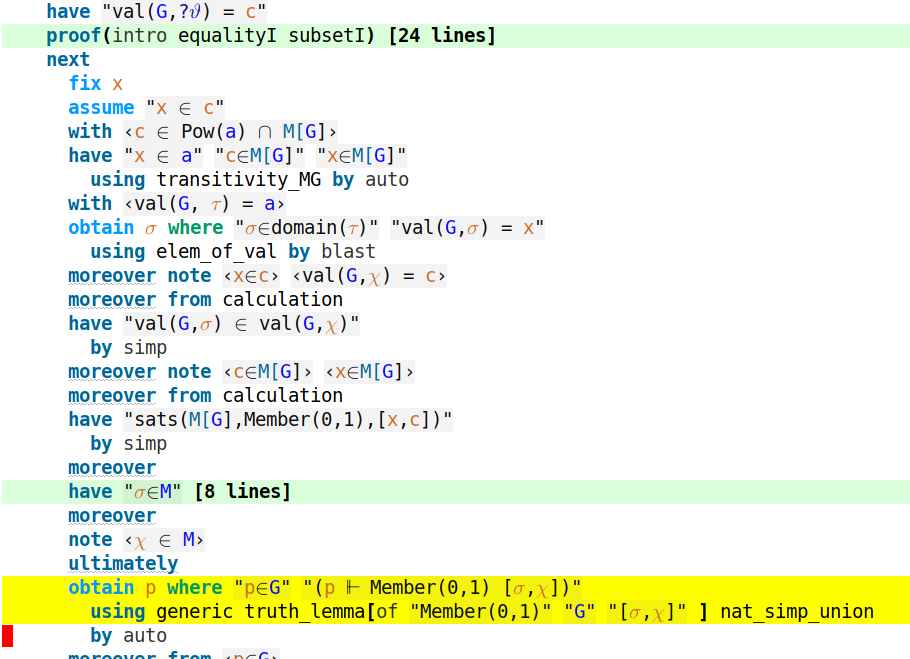
\includegraphics[scale=0.26]{isa_converted_17.png}}}%
    \only<18>{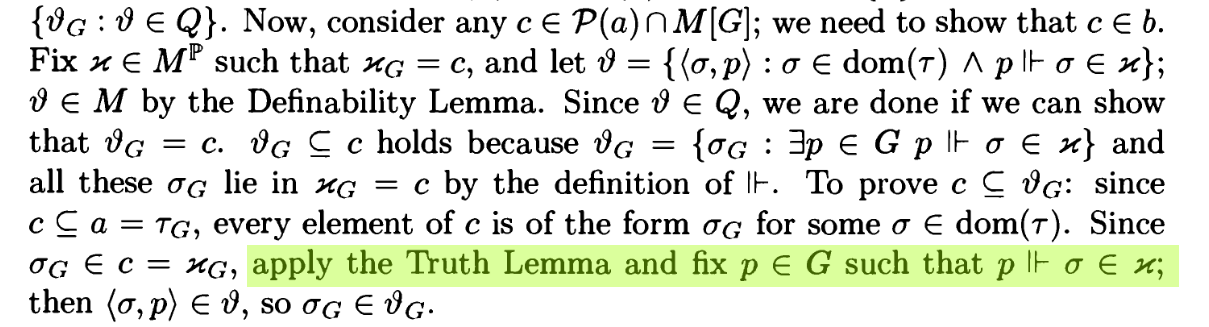
\includegraphics[scale=0.23]{kunen_powerset_18.png} \\ \fbox{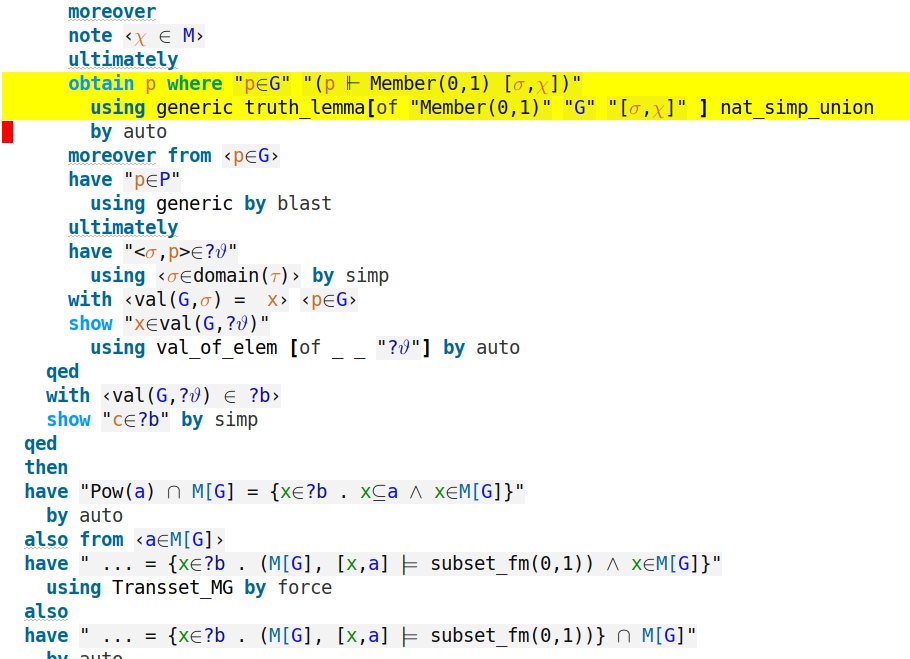
\includegraphics[scale=0.26]{isa_converted_18.png}}}%
    \only<19>{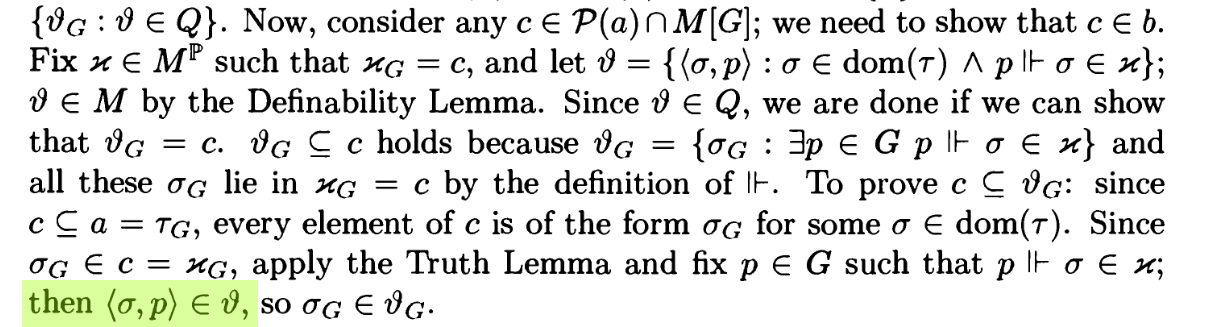
\includegraphics[scale=0.23]{kunen_powerset_19.png} \\ \fbox{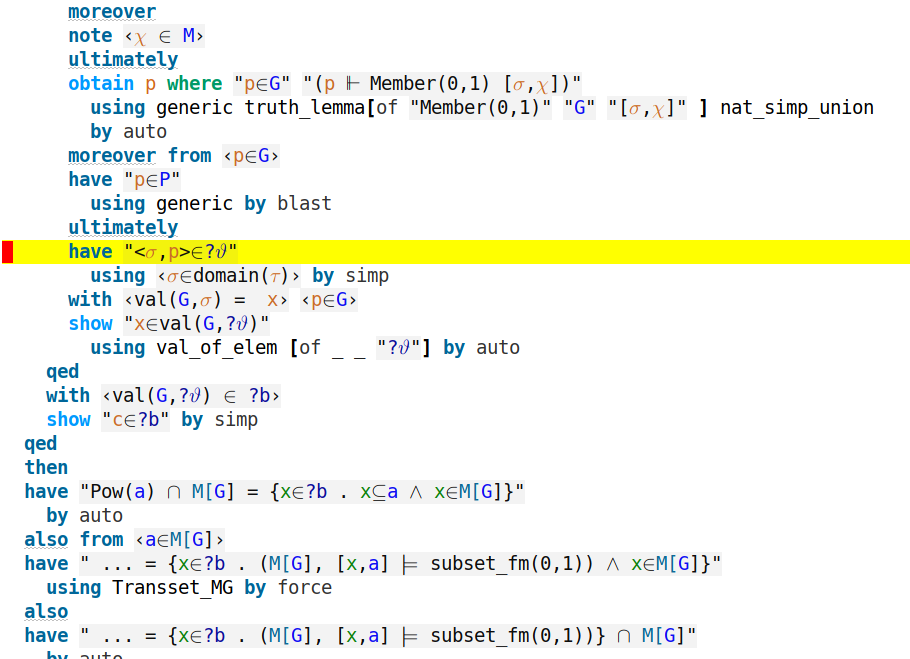
\includegraphics[scale=0.26]{isa_converted_19.png}}}%
    \only<20>{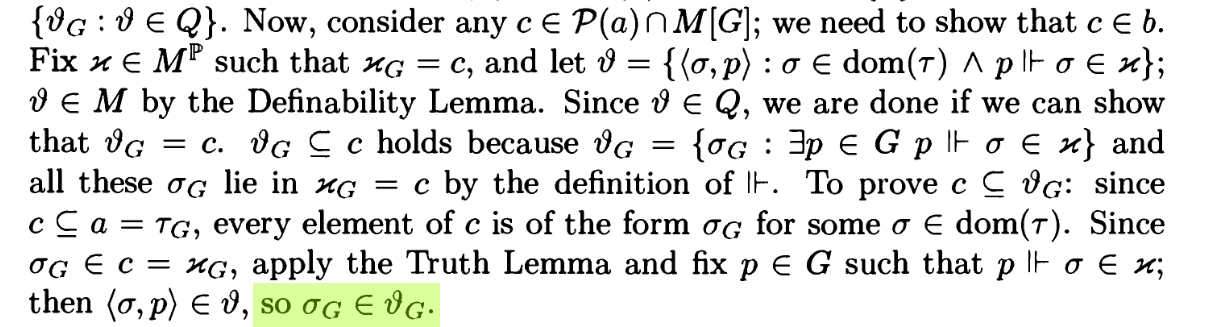
\includegraphics[scale=0.23]{kunen_powerset_20.png} \\ \fbox{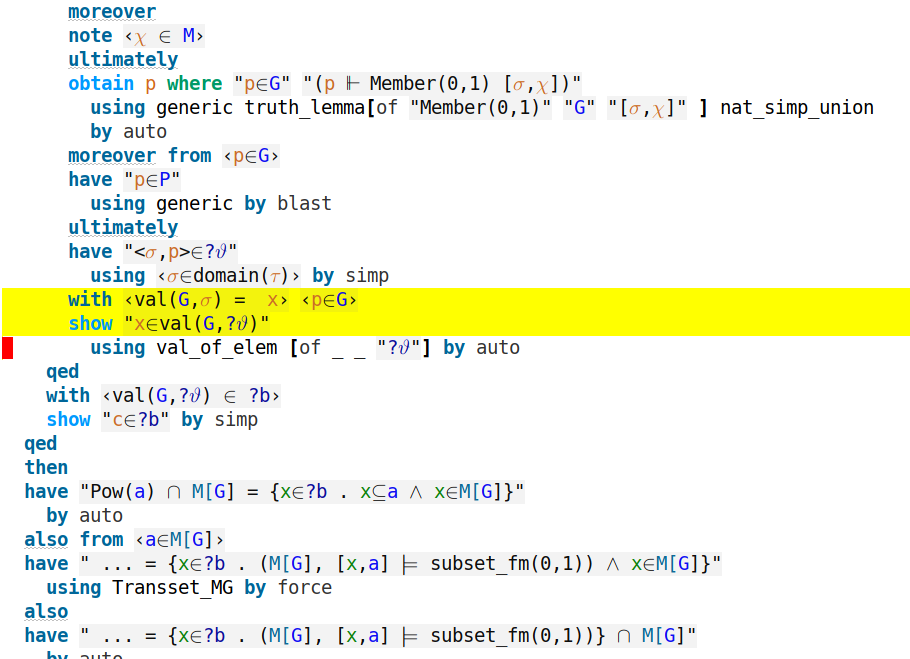
\includegraphics[scale=0.26]{isa_converted_20.png}}}%
  \end{center}
\end{frame}

%%%%%%%%%%%%%%%%%%%%%%%%%%%%%%%%%%%%%%%%%%%%%%%%%%%
\section{Looking forward}

\begin{frame}
  \frametitle{Looking forward}
  \begin{block}{Formalizing math}
    \begin{itemize}
    \item Cofinality, K\H{o}nig's Theorem, Shanin's $\Delta$-system Lemma.
    \item Forcing notion for adding $\kappa$ Cohen reals.
    \item Theorems on preservation of cardinals.
    \end{itemize}
  \end{block}
  \pause
  \begin{block}{Technical aids}
    \begin{itemize}
    \item Automatic relativization and proof of absoluteness of concepts.
    \item ``Relative functions'' (e.g., $\P^M$, $\card{\cdot}^M$, $\cf^M$).
    \end{itemize}
  \end{block}
\end{frame}

%-%-%-%-%-%-%-%-%-%-%-%-%-%-%-%-%-%-%-%-%-%-%-%-%-%
\begin{frame}
  \begin{shadowblock}{}
    \begin{center}
      {\Huge Thank you!}
    \end{center}
  \end{shadowblock}
\end{frame}

\begin{frame}
  \frametitle{References}
  \bibliographystyle{mi-estilo-else}
  \bibliography{../forcing_in_isabelle_zf}
\end{frame}

\begin{frame}
  \frametitle{Extra: Locale structure involving set models} 
             {  
               \renewcommand{\arraystretch}{1.5}               \begin{tabular}{rcl}
                 \texttt{forcing{\uscore}notion} & = & preorder $\PP$ with top. \\
                 \texttt{M{\uscore}ZF{\uscore}trans} & = & set model $M$ of the $\ZF$
                 axioms \alert{+}  $M$ transitive \\ 
                 \texttt{M{\uscore}ctm} & = &  \texttt{M{\uscore}ZF{\uscore}trans} \alert{+}
                 $M$ countable \\
                 \texttt{forcing{\uscore}data} & =  & \texttt{M{\uscore}ctm} \alert{+}
                 \texttt{forcing{\uscore}notion} $\PP\in M$\\
                 \texttt{separative{\uscore}notion} & = &
                 \texttt{forcing{\uscore}notion} \alert{+} $\PP$ separative \\
                 \texttt{M{\uscore}ctm{\uscore}separative} & = &
                 \texttt{forcing{\uscore}data} \alert{+}
                 \texttt{separative{\uscore}notion} \\
                 \texttt{G{\uscore}generic} & = & \texttt{forcing{\uscore}data} \alert{+} $G$ is $M$-generic
               \end{tabular} 
             }
\end{frame}

\begin{frame}
  \frametitle{Extra: More code review} 
  We only show the second inclusion $c\sbq \vartheta_G =
  \val(G,\vartheta)$ (the first one is proved in the
  course of the 24 folded lines).
\end{frame}

\againframe<13-20>{code-review}

\end{document}

%%% Local Variables: 
%%% mode: latex
%%% ispell-local-dictionary: "american"
%%% End: 
